\subsection{Data Layering}

We have a system which is able to support end-to-end encryption of data with permissions and access control. As an extension of this, we briefly consider how this data might be layered such that different parties see different views of data.

As an example, take the following JSON object in program code \ref{code:patient_record_json}. Let's assume this represents a record of a patient visiting a general practitioner.

\begin{listing}[H]
  \centering
  \begin{minted}{json}
{
  "doctor": {
    "id": 01234567,
    "name": "Dr. So So"
  },
  "metadata": {
    "created": "2017-01-01T10:05:00+00:00",
    "modified": "2017-01-01T10:11:12+00:00"
  },
  "notes": "..."
}
  \end{minted}
  \caption{
  	An example patient record
  }
  \label{code:patient_record_json}
\end{listing}


Now let's split the JSON object into three further JSON objects corresponding to the "doctor", "metadata", and "notes" properties. We could also do the same to the "doctor" and "metadata" objects. This would result in five separate JSON objects which, when combined, form the original JSON object. This is a recursively applied process.

\subsubsection{Storing data chunks}

Since the structure of a JSON object is representative of a tree, when evaluated as above, we can use this property to visualise the data as a file system:

\begin{figure}[H]
  \centering
  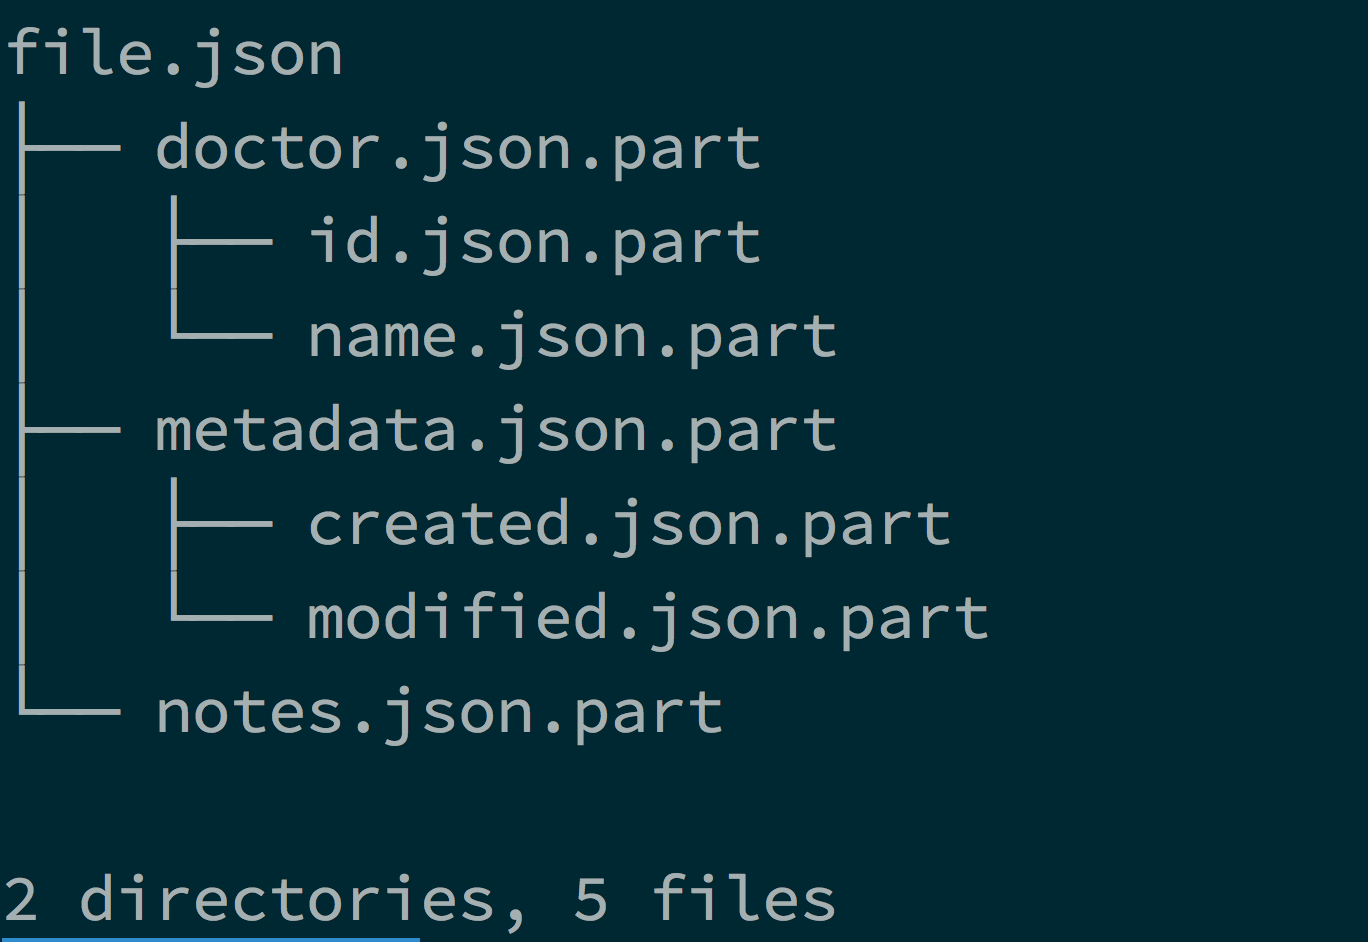
\includegraphics[width = 6cm]{images/json_file_structure.png} \\
  \caption{
  	JSON represented by file structure
  }{
    The use of the suffix '.part' denotes a file representing a property of the parent JSON object.
  }
  \label{fig:json_file_structure}
\end{figure}

We can transform the tree in figure \ref{fig:json_file_structure} into a Merkle tree by taking the hash of each file. Given the file content in program code \ref{code:patient_record_json} the resulting Merkle tree is shown in figure \ref{fig:json_merkle_tree}.

\begin{figure}[H]
  \centering
  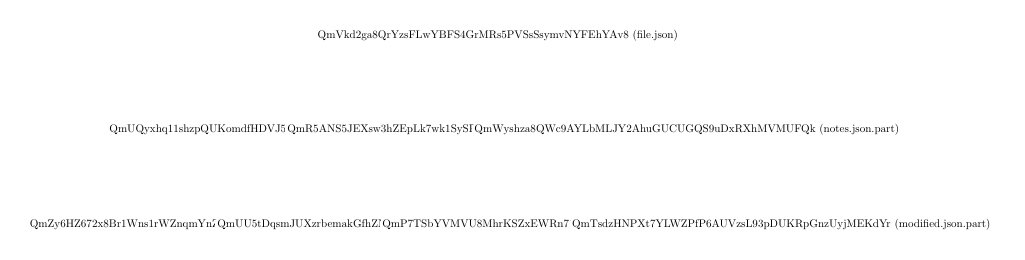
\begin{tikzpicture}[scale = 0.6, every node/.style={scale = 0.4}, every node/.append style={fill = white, rounded corners = 2pt, inner sep = 2pt, align = center}]

  \node at (0, 0) { QmVkd2ga8QrYzsFLwYBFS4GrMRs5PVSsSsymvNYFEhYAv8 (file.json) };
  
  \node at (-4, -2) { QmUQyxhq11shzpQUKomdfHDVJ5HGkrWZRFiPTLsc9hxK83 (doctor.json.part) };
  \node at (0, -2) { QmR5ANS5JEXsw3hZEpLk7wk1SySRDNnvBEdUu8RKgAybMz (metadata.json.part) };
  \node at (4, -2) { QmWyshza8QWc9AYLbMLJY2AhuGUCUGQS9uDxRXhMVMUFQk (notes.json.part) };
  
  \node at (-6, -4) { QmZy6HZ672x8Br1Wns1rWZnqmYnZ8ai1p6g5kmX2VkhDCr (id.json.part) };
  \node at (-2, -4) { QmUU5tDqsmJUXzrbemakGfhZN9edFZinA2i6iHiw3fsKim (name.json.part) };
  
  \node at (2, -4) { QmP7TSbYVMVU8MhrKSZxEWRn71F33RGSZaCPvSV47V2Anu (created.json.part) };
  \node at (6, -4) { QmTsdzHNPXt7YLWZPfP6AUVzsL93pDUKRpGnzUyjMEKdYr (modified.json.part) };

  \end{tikzpicture}
  \caption{
    Merkle tree of a JSON file
  }
  \label{fig:json_merkle_tree}
\end{figure}


Since IPFS is built on the notion of Merkle DAGs (Directed Acyclic Graph), this tree can be made by creating the "file.json" object on IPFS and recursively linking the aforementioned chunks.

Whilst a JSON file has been used in the above transformation, this extends well to any file type or encoding which is representable as a base64 (or similar) string. For example, if properties within the JSON were containers for binary data, the binary data needs to be converted to a base64 string prior to transforming the JSON to a Merkle tree.

\subsubsection{Permissions for data chunks}

Whilst splitting a file into chunks is relatively simple, permissioning the underlying data is more difficult.

Take the example whereby a storage contract owner uploads "file.json". This file is composed of three references to other files (it's properties), and two of those reference have another two files each (their properties). This requires the storage of five hashes, which (assuming directories are shown iff their underlying files are visible) results in $2^5$ possible permissions possibilities.

Unlike normal files where we want to observe the highest level of granularity (i.e. view individual files not clusters of files), we want to observe a very low level of granularity with file chunks (i.e. we want to see the parts of the file we can see compiled into a single file). The difficulty of this in terms of storage contracts is that we are unable to compose a complete file from file chunks within the compute layer (Ethereum) with present technology, given the inability for the computer layer to interact with non-deterministic services (side-effects).

We therefore need to assume that the client will rebuild the file on receipt of all it's (visible) parts. In doing so, we need an efficient way for the client to understand what it has access to when an individual requests a file. A function must be available on the storage contract which allows an identity to request the file paths contained within that file, and then use this to retrieve the individual data chunks.
